\documentclass[tikz,border=3pt]{standalone}
\usepackage[utf8]{inputenc}
\usepackage[T1]{fontenc}
\usepackage{lmodern}
\renewcommand{\familydefault}{\sfdefault}
\usepackage{sansmath}\sansmath
\usepackage{chemfig}
\usepackage{pgfplots}\pgfplotsset{compat=1.18,/pgf/number format/use comma,/pgf/number format/1000 sep={.}}
\usetikzlibrary{arrows.meta,calc,positioning,decorations.pathmorphing,patterns}
% paleta del sitio
\definecolor{nar}{HTML}{E8680C}\definecolor{narc}{HTML}{FFB35C}\definecolor{hielo}{HTML}{FFF3E8}
\definecolor{tinta}{HTML}{1D1D1F}\definecolor{gris}{HTML}{6E6E73}\definecolor{lila}{HTML}{7C5CF0}
\definecolor{azul}{HTML}{2F6FD6}\definecolor{menta}{HTML}{17A673}\definecolor{coral}{HTML}{E8342A}
\begin{document}
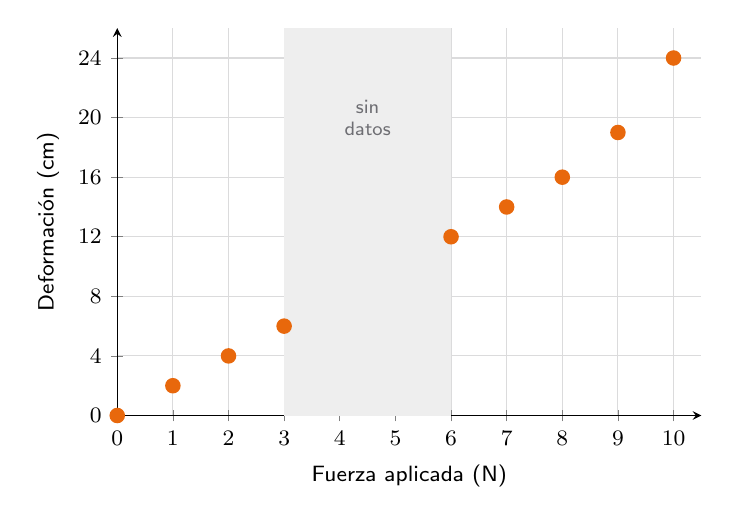
\begin{tikzpicture}[font=\footnotesize]
\begin{axis}[width=9cm,height=6.5cm,xmin=0,xmax=10.5,ymin=0,ymax=26,xtick={0,1,...,10},ytick={0,4,...,24},grid=major,grid style={gris!25},
  xlabel={Fuerza aplicada (N)},ylabel={Deformación (cm)},axis lines=left,every axis plot/.append style={thick}]
\fill[gris!12] (axis cs:3,0) rectangle (axis cs:6,26);
\node[text=gris,align=center,font=\scriptsize] at (axis cs:4.5,20) {sin\\datos};
\addplot[only marks,mark=*,mark size=2.4pt,color=nar] coordinates {(0,0)(1,2)(2,4)(3,6)(6,12)(7,14)(8,16)(9,19)(10,24)};
\end{axis}
\end{tikzpicture}
\end{document}
